% This is samplepaper.tex, a sample chapter demonstrating the
% LLNCS macro package for Springer Computer Science proceedings;
% Version 2.21 of 2022/01/12
%
\documentclass[runningheads]{llncs}
%
\usepackage[T1]{fontenc}
% T1 fonts will be used to generate the final print and online PDFs,
% so please use T1 fonts in your manuscript whenever possible.
% Other font encondings may result in incorrect characters.
%
\usepackage{graphicx}
% Used for displaying a sample figure. If possible, figure files should
% be included in EPS format.
%
% If you use the hyperref package, please uncomment the following two lines
% to display URLs in blue roman font according to Springer's eBook style:
%\usepackage{color}
%\renewcommand\UrlFont{\color{blue}\rmfamily}
%\urlstyle{rm}

\usepackage{amsmath}
\usepackage{marvosym}
\usepackage{hyperref}

% добавили авторы
\usepackage{multirow} 

\def\letter{$^{\textrm{(\Letter)}}$}

\begin{document}
%
\title{A Parallel Algorithm for Solving Global Optimization Problems and Its Application for Tuning Hyperparameters of AI Methods}
%
\titlerunning{A Parallel Algorithm for Tuning Hyperparameters}
% If the paper title is too long for the running head, you can set
% an abbreviated paper title here
%
\author{Marina Usova \letter \orcidID{0000-0002-0722-6884} \and
Ilya Lebedev\orcidID{0000-0002-8736-0652}  \and
Anton Shtanyuk\orcidID{0000-0003-1809-7173} \and
Evgeny Kozinov \orcidID{0000-0001-6776-0096} \and
Konstantin Barkalov \orcidID{0000-0001-5273-2471} 
}
%
\authorrunning{M. Usova et al.}
% First names are abbreviated in the running head.
% If there are more than two authors, 'et al.' is used.
%
\institute{Lobachevsky State University of Nizhni Novgorod, Nizhni Novgorod, Russia 
\email{usova@itmm.unn.ru}}
%
\maketitle              % typeset the header of the contribution
%
\begin{abstract}
%(рус.) В статье рассматривается параллельный алгоритм для решения задач глобальной оптимизации с частично определенной целевой функцией вида «черный ящик». Задачи такого вида возникают в процессе выбора оптимальных значений гиперпараметров методов машинного обучения и искусственного интеллекта. Алгоритм использует схему редукции размерности на основе кривых Пеано в сочетании с асинхронной схемой распараллеливания вычислений. Для демонстрации эффективности распараллеливания проведены вычислительные эксперименты в задаче настройки гиперпараметров методов искусственного интеллекта, используемых для предсказания значений временного ряда. 
The paper considers a parallel algorithm for solving global optimization problems with a partially defined objective function of the ``black box'' type. Such problems arise in the process of selecting optimal values of hyperparameters used in machine learning and artificial intelligence methods. The algorithm employs a dimensionality reduction scheme based on Peano curves in combination with an asynchronous scheme of parallel computing. To demonstrate the effectiveness of parallelization, computational experiments were conducted for the task of tuning the hyperparameters of artificial intelligence methods used to predict the values of a time series.

\keywords{Global Optimization  \and Multiextremal Functions \and Partially Defined Functions \and Hyperparameter Tuning \and  Time Series \and Artificial Intelligence.}
\end{abstract}
%
%
%

\section{Introduction}

%(рус.) В настоящее время методы машинного обучения и искусственного интеллекта используются во многих научных и прикладных областях. С их помощью успешно решаются задачи, которые еще недавно решались только классическими численными методами [ссылки]. 
Currently, machine learning and artificial intelligence methods are used in many academic and applied fields. They are successfully applied to address problems that until recently were solved only by classical numerical methods \cite{Blechschmidt2021,Seleznev2019,Xu2020}. 

%(рус.) В большинстве методов искусственного интеллекта имеются гиперпараметры, от выбора конкретных значений которых может зависеть эффективность их работы. Например, на качество классификации объектов с помощью метода опорных векторов, которое традиционно измеряется метрикой $F_1$ [ссылка], существенным образом влияют два параметра метода: коэффициент регуляризации и коэффициент ядра. При этом значения по умолчанию, ориентированные на средний случай, не будут являться наилучшими для конкретного класса решаемых задач. Подбор указанных параметров может значительно повысить значение целевой метрики качества.
Most artificial intelligence methods involve hyperparameters, and the choice of their specific values may determine their performance. For example, the quality of object classification using the support vector machine, which is traditionally measured by the $F_1$-score \cite{NIPS2015}, is significantly affected by two parameters of the method: the regularization coefficient and the kernel coefficient. However, the default values geared to the average case will not be the best for a particular class of problems to be solved. Appropriate selection of these parameters can significantly increase the value of the objective quality metric.

%(рус.) Таким образом, возникает the hyperparameter optimization (HPO) problem, которая с математической точки зрения является задачей глобальной оптимизации. Типичным является случай наличия не только непрерывных, но и категориальных параметров, т.е. возникает необходимость использования методы глобальной оптимизации, способные решать задачи со смешанными параметрами.
Thus, there arises the hyperparameter optimization (HPO) problem, which from the mathematical point of view is a global optimization problem. In this case, it is typical to have not only continuous but also categorical parameters (parameters having a prefixed set of values), i.e. there is a need to use global optimization methods capable of solving problems with mixed parameters. 
Such methods belonging to the class of metaheuristic and model-based algorithms are implemented in the well-known hyperparameter optimization frameworks Optuna \cite{optuna} and HyperOpt \cite{hyperopt}.

%(рус.) Традиционную сложность HPO problem составляет значительное время, требуемое для оценки критерия при конкретном сочетании параметров. Поэтому применение для данных задач метаэвристических алгоритмов, требующих большого числа поисковых испытаний, является ограниченным. Более перспективным здесь является использование детерминированных алгоритмов липшицевой оптимизации [Евтушенко, Сергеев, Стронгин], которые превосходят эвристические методы по качеству работы [Сергеев]. Для методов липшицевой глобальной оптимизации предложен ряд подходов к распараллеливанию, обеспечивающих эффективную работу на суперкомпьютерных системах [Евтушенко, Жилинскас, Гергель]. 
The traditional complexity of HPO problems is due to the considerable time required to evaluate a criterion for a particular combination of parameters. Therefore, metaheuristic algorithms, which require a large number of search trials, can find only a limited use for such problems. A more promising approach is to use deterministic Lipschitz optimization algorithms \cite{Evtushenko2013,Sergeyev2017,Strongin2000}, which are superior to heuristic methods in terms of performance quality \cite{Sergeyev2018}. For Lipschitz global optimization methods, a number of parallelization approaches have been proposed to ensure efficient operation in supercomputer systems \cite{Evtushenko2009,Gegrel2021,Paulavicius2011}. 

%
%
% !!!!!!!!!!!!!!! TO DO:: расширить обзор смежных исследований !!!!!!!!!!!!!
% "мало внимания обзору существующих методов и подходов для решения задачи оптимизации гиперпараметров"
%
%

%(рус.) Еще одной сложностью рассматриваемого класса задач HPO является наличие таких сочетаний значений гиперпараметров, при которых в некоторых (заранее не известных) подобластях области поиска исследуемый метод в принципе не работает. С такими значениями параметров невозможно корректно провести расчет и вычислить значение критерия эффективности. Данное явление можно интерпретировать как частичную определенность критерия в области поиска. В такой постановке HPO problem существенно усложняется, т.к. область допустимых сочетаний параметров является заранее неопределенной.
One more difficulty of the class of HPO problems being considered is the presence of such combinations of hyperparameter values for which the method under study does not work in principle in some (not known in advance) subdomains of the search domain. With such values of parameters it is impossible to perform the calculation correctly and calculate the value of the efficiency criterion. This phenomenon can be interpreted as partial definiteness of the criterion in the search domain. In such a formulation, the HPO problem becomes significantly more complicated, since the region of permissible combinations of parameters is undefined a priori.

%(рус.) Данная статья продолжает развитие подхода к параллельному решению задач липшицевой глобальной оптимизации, предложенного в работах [наши работы]. Новым элементом является сочетание способов распараллеливания и предложенной в [Усова] схемы работы с частично вычислимыми функциями. Основная часть публикации имеет следующую структуру. В Section 2 приведена математическая постановка решаемой задачи. Section 3 содержит описание параллельного алгоритма глобального поиска. В Section 4 описан способ решения задач со смешанными (дискретными и непрерывными) параметрами, а также обсуждается способ работы с функциями, определенными не во всей области поиска. Section 5 содержит результаты вычислительных экспериментов, демонстрирующих эффективность предлагаемого подхода при решении задачи оптимизации гиперпараметров методов прогнозирования значений временного ряда.
This paper continues to develop the approach to solving Lipschitz global optimization problems in parallel \cite{Barkalov2018,Gegrel2021,Strongin2018}. The new element is the combination of parallelization methods and the scheme for handling partially computable functions proposed in \cite{Usova2024}. The main part of the publication has the following structure.  Section \ref{sec:PS} presents the mathematical formulation of the problem to be solved. Section \ref{sec:PA} contains a description of the parallel global search algorithm. Section \ref{sec:MP} describes the method for solving problems with mixed (discrete and continuous) parameters, and also discusses the method for handling functions that are not defined in the entire search domain. Section \ref{sec:RCE} gives the results of computational experiments demonstrating the effectiveness of the proposed approach in solving the problem of optimizing the hyperparameters of time series forecasting methods.

\section{Problem Statement}\label{sec:PS}
%(рус.) В начале рассмотрим задачу оптимизации в простой постановке, только с непрерывными параметрами. Пусть требуется найти минимум функции $\phi(y)$, определенной в области $D$
First, consider the optimization problem in a simpler formulation, with only continuous parameters. Let it be required to find the minimum of the function $\phi(y)$ defined in the domain $D$

\begin{equation} \label{problem}
\phi(y^*) = \min \left\{\phi(y): y \in D, g_i(y) \leq 0, 1 \leq i \leq m\right\}, 
\end{equation}
\[ D=\left\{ y \in R^N: a_i \leq y_i \leq b_i, \; 1 \leq i \leq N\right\}. \]

%(рус.) Будем предполагать, что целевая функция $\phi(y)$ является многоэкстремальной удовлетворяет условию Липшица
We will assume that the objective function $\phi(y)$ is multiextremal and satisfies the Lipschitz condition
\begin{equation}\label{lipschitz} 
| \phi (y_1)-\phi (y_2) | \leq L \| y_1-y_2 \|, \; y_1,y_2 \in D.
\end{equation}

%(рус.) Известным способом решения задач липшицевой глобальной оптимизации является их сведение (явное или неявное) к решению одномерных задач. Такое сведение может быть выполнено, например, на основе использования диагональных или симплексных разбиений области поиска [ссылки].
A well-known way to solve Lipschitz global optimization problems is to reduce them (explicitly or implicitly) to the solution of one-dimensional problems. Such a reduction can be performed, for example, by using diagonal or simplicial partitions of the search domain \cite{PaulaviciusZilinskas2014,Sergeyev2017}.

%(рус.) В нашем исследовании мы используем схему редукции размерности на основе кривых Пеано y(x), однозначно и непрерывно отображающих отрезок [0,1] на N-мерный гиперкуб D [ссылки]. В результате такой редукции многомерная задача глобальной оптимизации (1) сводится к одномерной задаче
In our research, we use a dimensionality reduction scheme based on Peano curves $y(x)$ that uniquely and continuously map the segment $[0,1]$ to an $N$-dimensional hypercube $D$ \cite{Strongin2000}. As a result of this reduction, the multidimensional global optimization problem (\ref{problem}) reduces to a one-dimensional problem

\begin{equation} \label{reduced_problem}
\min \left\{\phi(y(x))\right\} = \min \left\{\phi(y)\right\}, x \in [0,1],  y \in D.
\end{equation}

%(рус.) Использование кривых Пеано сохраняет ограниченность разностей функции. Если исходная функция φ(x) удовлетворяла условию Липшица, то редуцированная одномерная функция φ(y(x)) из (3) будет удовлетворять условию Гёльдера
By using Peano curves, the boundedness of the function differences is preserved. If the original function $\phi(y)$ satisfied the Lipschitz condition, then the reduced one-dimensional function $\phi(y(x))$ from (\ref{reduced_problem}) will satisfy the H{\"o}lder condition
\begin{equation}\label{holder} 
| \phi (y(x'))-\phi (y(x'')) | \leq H | x' - x''|^\frac{1}{N},
\end{equation}
%(рус.) где константа H определяется соотношением H=2L√(N+3), а L есть константа Липшица из (2). 
where the constant $H$ is defined by the relation $H=2L\sqrt{N+3}$, and $L$ is the Lipschitz constant from (\ref{lipschitz}).  

%(рус.) Таким образом, проведение испытания в точке x^k  ∈ [0,1] подразумевает:
	%(рус.) вычисление image y^k   = y(x^k ) in accordance with the mapping y(x);
	%(рус.) вычисление значения функции z^k  =φ(y^k ).
Thus, performing a trial at a point $x^k \in [0,1]$ involves:
\begin{itemize}
    \item calculating the image $y^k=y(x^k)$ in accordance with the mapping $y(x)$;
    \item calculating the value of the function $z^k=\phi(y^k)$.
\end{itemize}

%
%
% ЗАМЕЧАНИЕ: "не понятно назначение рисунка, т.к. читателю должен быть знаком общий вид одномерной функции"
% Graph of the one-dimensional function after dimensionality reduction     of multiextremal objective function ????
%
%

\begin{figure}
\center
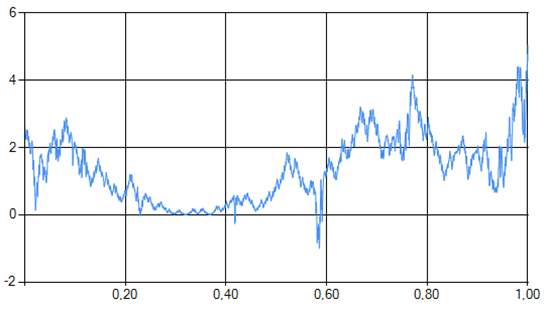
\includegraphics[width=0.8\textwidth]{fig1.png}
\caption{Graph of the one-dimensional function after dimensionality reduction of multiextremal objective function.} \label{fig1}
\end{figure}

%(рус.) При численной реализации оптимизационных алгоритмов используется развертка, приближающая истинную кривую Пеано с заданной точностью, которая определяется желаемой точностью поиска глобального экстремума. В качестве примера на Fig. 1 приведена одномерная функция, получающаяся в результате редукции двумерной задачи. График демонстрирует сложную структуру получающейся одномерной функции.
In the numerical implementation of optimization algorithms, an evolvent is used to approximate the true Peano curve with a given accuracy, which is determined by the desired accuracy of the search for the global extremum. As an example, Fig.~\ref{fig1} shows a one-dimensional function resulting from the reduction of a two-dimensional problem. The graph demonstrates the complex structure of the resulting one-dimensional function.

\section{Parallel asynchronous global search algorithm}\label{sec:PA}

%(рус.) К настоящему времени разработаны различные подходы к организации параллельных вычислений для различных численных алгоритмов. Однако при решении задач многомерной многоэкстремальной оптимизации известные способы или не обеспечивают должного эффекта, или вообще не применимы. Например, один из основных способов организации параллельных вычислений состоит в разделении области решения задачи между процессами и параллельного решения задачи в этих подобластях. Но в случае решения задач глобальной оптимизации такой подход будет неэффективным, поскольку при разделении области поиска только небольшая часть процессов будет работать в подобласти с искомым глобальным минимумом, все же остальные будут работать в подобластях, в которых отсутствует глобальный минимум исходной задачи.
Various approaches to organizing parallel computations for various numerical algorithms have been developed to date \cite{Voevodin2015}. However, when solving multidimensional multiextremal optimization problems the known methods either do not provide proper effect or are not applicable altogether. For example, one of the main ways of organizing parallel computations consists in dividing the problem solving domain between processes and solving the problem in parallel in these subdomains. However, this approach will be inefficient for solving global optimization problems, because when dividing the search domain, only a small part of the processes will run in the subdomain with the desired global minimum, while the rest will run in the subdomains in which there is no global minimum of the original problem.

%(рус.) Более продуктивный подход к распараллеливанию основан на изменении схемы последовательного алгоритма для параллельного выполнения нескольких испытаний. Отметим, что в задачах рассматриваемого класса (задачах настройки гиперпараметров методов машинного обучения) типичной является ситуация, когда целевая функция имеет разную трудоемкость вычисления в разных точках области поиска. В таких задачах распределение точек испытаний между параллельно работающими процессами должно происходить асинхронно, по запросу. В самом деле, в случае синхронного проведения испытаний часть процессов (которые проводят испытаний в «легкой» подобласти) закончит вычисления и будет простаивать, дожидаясь окончания расчетов остальных процессов (которым достались точки из «сложной» подобласти). 
A more productive approach to parallelization is based on changing the sequential algorithm scheme for performing several trials in parallel. Note that in the problems of the class under consideration (problems of hyperparameter tuning for machine learning methods) a typical situation is when the objective function has different computational complexity at different points of the search domain. In such problems, the distribution of trial points between parallel processes should be performed asynchronously, on demand. Actually, in case of synchronous trials, some processes (which perform trials in the ``easy'' subdomain) will finish calculations and will idle, waiting for the rest of the processes (which were assigned the points from the ``difficult'' subdomain) to finish calculations.

%(рус.) В асинхронном алгоритме глобального поиска реализована схема распараллеливания вида ''master/worker''. При описании алгоритма будем предполагать, что в нашем распоряжении имеется p+1 вычислительный процесс: один процесс-мастер и p рабочих процессов. Процесс-мастер организует сбор, накопление и обработку поисковой информации (результатов выполненных испытаний). На ее основе мастер вычисляет точки новых испытаний и распределяет их по процессам-рабочим. Процессы-рабочие получают от мастера точки, проводят в них новые испытания и отсылают мастеру их результаты.
We used in our study an asynchronous global search algorithm, which implements a parallelizing scheme of the ``master/worker'' type. When describing the algorithm we will assume that we have at our disposal $p+1$ process: one master process and $p$ worker processes. The master process organizes the collection, accumulation and processing of search information (results of performed trials). Based on this information, the master calculates the points of new trials and distributes them to the worker processes. The worker processes receive the points from the master, perform new trials in these points and send their results to the master.

%(рус.) На первой итерации алгоритма процесс-мастер (равномерно или случайно) выбирает p различных внутренних точек области поиска {x^1,x^2,…,x^p }, x^i∈(0,1),i=1,…,p, и рассылает точки испытаний по процессам-рабочим для выполнения испытаний в них. Правила работы процесса-мастера на любой из следующих итераций состоят в следующем. 
At the first iteration of the algorithm, the master process selects (uniformly or randomly) $p$ different internal points of the search domain ${x^1, x^2, ..., x^p}, x^i \in (0,1), i=1, ..., p$, and distributes the trial points to the worker processes to perform trials in those points. The rules for the master process at any of the subsequent iterations are as follows. 

%(рус.) Пусть проведено k испытаний, их результаты получены и обработаны мастером, а на текущей итерации процессы-рабочие проводят испытания в точках множества S_k  = {x^(k+1),x^(k+2),…,x^(k+p) }, т.е. в этих точках испытания уже начались, но еще не завершены. Как только один из процессов-рабочих завершает проведение испытания в некоторой точке (например, x^(k+1)), он пересылает процессу-мастеру результаты испытания. Получив от рабочего процесса результаты испытания и обработав их мастер, в свою очередь, выбирает для него точку нового испытания x^(k+p+1) в соответствии со следующими правилами.
Suppose $k$ trials have been performed, the master has received and processed their results, and during the current iteration the worker processes perform trials at the points of the set $S_k={x^{k+1}, x^{k+2},..., x^{k+p}}$, i.e. the trials have already started at these points but have not yet been completed. As soon as one of the worker processes completes a trial at some point (e.g. $x^{k+1}$), it forwards the results of the trial to the master process and the point is excluded from the set $S_k$. After receiving the trial results from the worker process and processing them, the master process in turn selects a new trial point $x^{k+p+1}$ for the worker process according to the following rules.

\begin{enumerate}
%(рус.) 1. Перенумеровать в порядке возрастания все точки X_k  = {x^1,x^2,…,x^(k+p)  }, в которых либо проведены, либо проводятся испытания, т.е.
\item Renumber, in ascending order, all the points $X_k={x^1,x^2,...,x^{k+p} }$ at which trials have either been carried out or are being carried out, i.e.
\[
0 = x_1 \leq x_2 \leq ... \leq x_{k+p} = 1,
\]
%(рус.) и сопоставить им значения z_i=φ(y(x_i )) , 1≤i≤k, вычисленные в этих точках, а также индекс v_i=v(x_i ), определяемый по правилу
and assign to them the values $z_i = \phi(y(x_i)), 1 \leq i \leq k$ calculated at these points, as well as the index $v_i = v(x_i)$ determined by the rule

\begin{equation}\label{rule_points_index} 
v_i=v(x_i)=
\begin{cases}
    0,     & \quad \text{if } x_i \text{ is boundary point},\\
    1,     & \quad \text{if } x_i \text{ is internal point}.
\end{cases}
\end{equation}
%(рус.) Точки x_0=0 и x_(k+p)=1 введены дополнительно (значения z_0 и z_(k+p) не определены) для удобства последующих обозначений.
The points $x_0=0$ and $x_{k+p}=1$ are additionally introduced (the values $z_0$ and $z_{k+p}$ are not defined) for the convenience of subsequent designations.

%(рус.) 2. Вычислить значения
\item Calculate the values
\[
M_1= \max \left\{ \frac{|z_i - z_{i - 1}|}{(x_i - x_{i - 1})^\frac{1}{N}}: x_{i-1} \notin S_k, x_i \notin S_k, 2 \leq i \leq k+p \right\},
\]
\[
M_2= \max \left\{ \frac{|z_{i+1} - z_{i - 1}|}{(x_{i+1} - x_{i - 1})^\frac{1}{N}}: x_{i} \in S_k, 2 \leq i < k+p \right\},
\]
\[
M= \max \left\{ M_1, M_2 \right\},
\]
%(рус.) где z_i=f(x_i ), if x_i  ∉  S_k,1≤ i≤ k+p. Значения z_i в точках x_i∈S_k являются неопределенными, т.к. испытания в этих точках еще не завершены. Если значение M получилось равным 0, то положить M=1.
where $z_i=\phi(y(x_i))$, if $x_i \notin S_k, 1 \leq i \leq k+p$. The values $z_i$ at the points $x_i \in S_k$ are undefined because the trials at these points have not yet been completed. If the value $M$ turns out to be equal to $0$, then assume $M=1$.

%(рус.) 3. Определить текущее лучшее значение целевой функции
\item Determine the current best value of the objective function
\begin{equation}\label{cur_best_val} 
z^* = \min \left\{ \phi(y(x_i)): 1 \leq i \leq k \right\}.
\end{equation}

%(рус.) 4. Каждому интервалу (x_(i-1),x_i ),x_(i-1)  ∉ S_k,x_i  ∉ S_k,2≤ i≤ k+p, поставить в соответствие число R(i), которое называется характеристикой интервала и вычисляется по формуле
\item Assign a number $R(i)$ to each interval $(x_{i-1}, x_i), x_{i-1} \notin S_k, x_i \notin S_k, 2 \leq i \leq k+p$, which is called the interval characteristic and is calculated using the formula
\begin{equation}\label{characteristic}
R(i)=
\begin{cases}
    \Delta_i+\frac{(z_i-z_{i-1})^2}{(rM)^2\Delta_i} - 2 \frac{(z_i+z_{i-1}-2z^*)}{rM},   & \quad v(x_i)=v(x_{i-1})=1,\\
    2\Delta_i- 4 \frac{(z_i-z^*)}{rM},   & \quad v(x_i)=1, v(x_{i-1})=0,\\
    2\Delta_i- 4 \frac{(z_{i-1}-z^*)}{rM},       & \quad v(x_i)=0, v(x_{i-1})=1,\\
\end{cases}
\end{equation}
%(рус.) где Δ_i  =(x_i-x_(i-1) )^(1/N) , and r>1 – параметр алгоритма.
where $\Delta_i=(x_i-x_{i-1})^\frac{1}{N}$, and $r>1$ is the parameter of the algorithm.

%(рус.) 5. Выбрать интервал [x_(t-1),x_t ], которому соответствует максимальная характеристика, т.е.
\item Choose the interval $[x_{t-1}, x_t]$ to which the maximum characteristic corresponds, i.e.
\[
R(t)= \max \left\{ R(i): x_{i-1} \notin S_k, x_i \notin S_k, 2 \leq i \leq k+p\right\}.
\]

%(рус.) 6. Вычислить точку проведения нового испытаний x^{k+p+1} ∈ (x_(t-1),x_t ) в соответствии с формулами
\item Calculate the point of the new trial $x^{k+p+1} \in (x_{t-1}, x_t)$ according to the formulas
\begin{equation}\label{new_point_1} 
x^{k+p+1} = \frac{x_t+x_{t-1}}{2}, \text{ if } v(x_{t-1}) \neq v(x_t),
\end{equation}
\begin{equation}\label{new_point_2} 
x^{k+p+1} = \frac{x_t+x_{t-1}}{2}-\frac{\textit{sign}{(z_t-z_{t-1})}}{2r} \left[ \frac{|z_t-z_{t-1}|}{M} \right]^N,
\end{equation}
if $v(x_{t-1})=v(x_t)$.
%(рус.) Сразу после вычисления точки очередного испытания процесс-мастер добавляет ее в множество S и пересылает процессу-рабочему, который начинает проведение испытания в ней.
Immediately after calculating the point of the next trial, the master process adds it to the set $S$ and forwards it to the worker process, which starts a trial there.
\end{enumerate}

%(рус.) Работа алгоритма завершается, если в мастер-процессе выполняется одно из двух условий: Δ_t<ϵ or k+p>K_max. Выполнение первого неравенства соответствует остановке алгоритма по заданной точности поиска 0<ϵ<1, выполнение второго – по заданному числу испытаний K_max>0.
The algorithm is terminated if one of two conditions is met in the master process: $\Delta_t< \varepsilon$ or $k+p>K_{max}$. The fulfillment of the first inequality corresponds to stopping the algorithm for a given search accuracy $0< \varepsilon <1$, and the fulfillment of the second one corresponds to a given number of trials $K_{max}>0$.

%(рус.) Теоретические основы алгоритма, а также примеры его применения приведены в работах [ссылки].
The theoretical background of the algorithm as well as examples of its application are given in  \cite{Barkalov2018,Barkalov2023,Gubaydullin2021,Strongin2020}.

\section{Handling mixed parameters and functions that are not defined everywhere}\label{sec:MP}

%(рус.) Теперь рассмотрим задачу оптимизации в более сложной постановке. Пусть целевая функция задачи зависит от двух векторов параметров: вектора y∈D,  и вектора u∈U, т.е.
Now consider the optimization problem in a more complex setting. Let the objective function of the problem depend on two vectors of parameters: vector $y \in D$, and vector $u \in U$, i.e.

\begin{equation}\label{mixed_problem} 
\phi(y^*, u^*) = \min \left\{\phi(y, u): y \in D, u \in U\right\}.
\end{equation}

%(рус.) Задача оптимизации в такой постановке является математической моделью проблемы поиска наилучшей комбинации гиперпараметров методов искусственного интеллекта. Здесь D соответствует области изменения непрерывных гиперпараметров, а множество U содержит возможные сочетания категориальных гиперпараметров.
The optimization problem in this formulation is a mathematical model of the problem of finding the best combination of hyperparameters of artificial intelligence methods. Here, $D$ corresponds to the region of variation of continuous hyperparameters, and the set $U$ contains possible combinations of categorical hyperparameters.

%(рус.) Задачу со смешанными параметрами можно свести к решению взаимосвязанного набора задач с непрерывными параметрами. Занумеруем целыми числами все различные комбинации категориальных параметров, т.е. сопоставим каждому номеру s вектор u_s. Тогда (10) можно переписать в виде 
A problem with mixed parameters can be reduced to solving an interrelated set of problems with continuous parameters. Let us number all different combinations of categorical parameters with integers, i.e., let us assign to each number $s$ a vector $u_s$. Then (\ref{mixed_problem}) can be rewritten as 

\begin{equation}\label{mixed_problem_2} 
 \min \left\{\phi(y, u)\right\} = \min_{s \in \{1, ..., S\}} \left\{\phi(y, u_s): y \in D\right\}.
\end{equation}

%(рус.) Используя схему редукции размерности с помощью кривых Пеано y(x), каждой задаче минимизации из (11) можно сопоставить одномерную задачу минимизации, т.е. сформировать множество одномерных задач
Using the dimensionality reduction scheme with Peano curves $y(x)$, each minimization problem from (\ref{mixed_problem_2}) can be matched with a one-dimensional minimization problem, i.e. we can obtain a set of one-dimensional problems
\begin{equation}\label{reduced_mixed_problem} 
 \min \left\{\phi(y(x), u_s): x \in [0,1]\right\}, s \in \{1, ..., S\}.
\end{equation}

%(рус.) Если теперь ввести в рассмотрение отображение
If we now introduce the mapping
\[
Y(x) = y(x-E(x)), x \in [0, S],
\]
%(рус.) переводящее любую точку интервала [0,S] на область D (обозначение E(x) соответствует целой части числа x) и определить функцию
which translates any point of the interval $[0,S]$ to the domain $D$ (the notation $E(x)$ corresponds to the integer part of the number $x$) and define the function
\[
f(x)=\phi(Y(x), u_{E(x) + 1}), x \in [0, S],
\]
%(рус.) можно переформулировать задачу (11) как
we can reformulate problem (\ref{reduced_mixed_problem} ) as
\begin{equation}\label{reduced_mixed_problem_2} 
 \min \left\{f(x): x \in [0,S]\right\}.
\end{equation}

%(рус.) Применяя к решению задачи (12) алгоритм глобального поиска, мы найдем решение задачи (10). 
Applying the global search algorithm to solve problem (\ref{reduced_mixed_problem_2}), we will find a solution to problem (\ref{mixed_problem}). 

%(рус.) Отметим, что функция f(x), вообще говоря, может иметь разрывы в целочисленных точках x_i  = i. Так как эти точки известны заранее, их можно на первой итерации добавить в информационную базу алгоритма со значением индекса равным 0. В соответствии с правилами алгоритма, в процессе его работы не будет возникать интервалов, обе граничные точки которых имеют нулевой индекс, и правила вычисления характеристик (7) и точки нового интервала (8)-(9) будут валидными.
Note that the function $f(x)$, in general, can have discontinuities at integer points $x_i=i$. Since these points are known in advance, they can be added to the information base of the algorithm at the first iteration with an index value equal to $0$. According to the rules of the algorithm, during its operation there will be no intervals with both boundary points having zero index, and the rules for calculating the characteristics (\ref{characteristic}) and the points of the new interval (\ref{new_point_1})-(\ref{new_point_2}) will be valid.

%(рус.) Однако в рассматриваемых задачах настройки гиперпарметров целевая функция может быть не определена в некоторых (заранее неизвестных) точках области поиска. Это может приводить возникновению интервалов, у которых обе граничных точки имеют нулевой индекс, т.е. значение целевой функции в них не определено. Возможный подход к обработке таких интервалов состоит в использовании на шаге 4 алгоритма для вычисления характеристики вместо формулы (7) следующей формулы
However, in the hyperparameter tuning tasks under consideration, the objective function may be undefined in some (previously unknown) points in the search domain. This may give rise to intervals where both boundary points have a zero index, i.e. the value of the objective function is undefined in these points. A possible approach to processing such intervals is to use the following formula at step 4 of the algorithm to calculate the characteristic instead of formula (\ref{characteristic})

\begin{equation}\label{characteristic_2}
R(i)=
\begin{cases}
    \Delta_i+\frac{(z_i-z_{i-1})^2}{(rM)^2\Delta_i} - 2 \frac{(z_i+z_{i-1}-2z^*)}{rM},   & \quad v(x_i)=v(x_{i-1})=1,\\
    2\Delta_i- 4 \frac{(z_i-z^*)}{rM},   & \quad v(x_i)=1, v(x_{i-1})=0,\\
    2\Delta_i- 4 \frac{(z_{i-1}-z^*)}{rM},       & \quad v(x_i)=0, v(x_{i-1})=1,\\
    \alpha(1-1/r)^2\Delta_i,       & \quad v(x_i)=0, v(x_{i-1})=0,\\
\end{cases}
\end{equation}

%(рус.) В последнем выражении 〖 (1-1\/r)〗^2 ∆_i соответствует нижней оценке характеристики интервала, содержащего текущее найденное решение z^* из (6) (вывод данной оценки см. в [ссылка]). А параметр 0<α<1 соответствует априорный оценке доли объема области поиска, в которой значения функции являются неопределенными. 
In the latter expression, $\alpha(1-1/r)^2\Delta_i$ corresponds to the lower estimate of the characteristic of the interval containing the current solution $z^*$ found from (\ref{cur_best_val}) (see \cite{Strongin2020} for the derivation of this estimate). The parameter $0<\alpha<1$ corresponds to an a priori estimate of the portion of the search domain volume in which the function values are undefined.  

%(рус.) Также требуется дополнить правило выбора точки нового испытания для обработки ситуаций, когда обе граничные точки имеют нулевой индекс:
It is also necessary to supplement the rule for selecting a new trial point to handle situations where both boundary points have a zero index:
\begin{equation}\label{new_point_1_2} 
x^{k+p+1} = \frac{x_t+x_{t-1}}{2}, \text{ if } v(x_{t-1}) \neq v(x_t) \text{ or } v(x_{t-1})=v(x_t)=0,
\end{equation}
\begin{equation}\label{new_point_2_2} 
\begin{split}
x^{k+p+1} = \frac{x_t+x_{t-1}}{2}-\frac{\textit{sign}{(z_t-z_{t-1})}}{2r} \left[ \frac{|z_t-z_{t-1}|}{M} \right]^N, \\
\text{if }  v(x_{t-1})=v(x_t) = 1.
\end{split}
\end{equation}


%(рус.) Формула (14) будет применяться, если значения как минимум в одной из граничных точек интервала значения целевой функции не определены, тогда как формула (15) будет использоваться только в случае, когда значения целевой функции вычислены в обоих точках.
Formula (\ref{new_point_1_2}) will be used if the values in at least one of the boundary points of the objective function value interval are undefined, while formula (\ref{new_point_2_2}) will be used only when the values of the objective function are calculated at both points.

\section{Results of computational experiments}\label{sec:RCE}

%(рус.) Рассмотренные в статье методы реализованы в iOpt parallel solver, разрабатываемом в ННГУ им. Н.И. Лобачевского и предназначенном для решения многомерных задач глобальной оптимизации. 
The methods considered in this paper are implemented in the iOpt parallel solver \cite{iOptURL}, which is being developed at Lobachevsky State University of Nizhni Novgorod  for solving multidimensional global optimization problems.

%(рус.) В качестве модельной задачи нами была использована задача настройки гиперпараметров методов предсказания значений временного ряда (Time Series Forecasting). В качестве исходных данных был использован датасет montly beer prodaction [5.1], содержащий 476 valid data points. 
We used the task of hyperparameter tuning for time series forecasting methods as a model problem. The monthly beer production dataset \cite{MonthlyBeerDataset,MonthlyBeerArticle} containing 476 valid data points was used as input data. 

%(рус.) Для решения задачи предсказания значений временного ряда мы использовали фреймворк машинного обучения FEDOT [5.2, 5.2.1] (open-source framework for automated modeling and machine learning (AutoML) problems). FEDOT поддерживает полный цикл решения задачи, включающий препроцессинг, выбор модели, настройку, кроссвалидацию и т.д. Фреймворк использует ML-модели, в основном из библиотек sklearn, statsmodels и keras, а также интегрирован с GOLEM open-source framework.
To solve the problem of predicting time series values, we used the machine learning framework FEDOT \cite{FEDOT,nikitin2022automated} (open-source framework for automated modeling and machine learning problems). FEDOT supports the full problem solving cycle including preprocessing, model selection, tuning, cross validation, etc. The framework uses ML models, mainly from the sklearn, statsmodels and keras libraries, and is integrated with the GOLEM open-source framework.

%(рус.) Построенный с использованием FEDOT pipeline включает в себя комбинацию из двух преобразований: lagged и cgru. Lagged-преобразование выполняется путем взятия значения переменной в предыдущий момент времени и включения его в модель в качестве признака в текущий момент времени. Для этого данные временного ряда сдвигаются на определенное количество шагов, которые называются лагом или временной задержкой. В качестве используемой нейронной сети будет выступать рекуррентная сеть (GRU), использующая свертку (CGRU).
The pipeline constructed using FEDOT involves a combination of two transformations: \textit{lagged} and \textit{cgru}, Fig.~\ref{fig2}. Lagged transformation is performed by taking the value of a variable at a previous point in time and incorporating it into the model as a feature at the current point in time. For this purpose, the time series data is shifted by a certain number of steps, which are called  a lag  or time delay. A recurrent network (GRU) using convolution (CGRU) will serve as the neural network.

%
%
% TO DO: "возможно, вместе с pipeline, стоило бы проиллюстрировать архитектуру сети"
%
%
%

\begin{figure}
\center
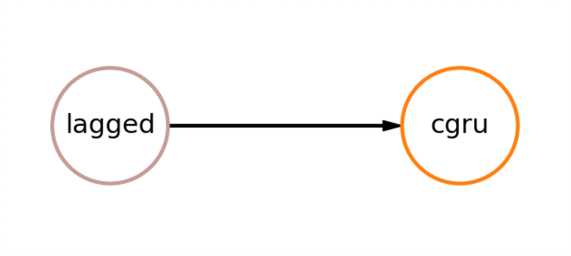
\includegraphics[width=0.5\textwidth]{fig2.png}
\caption{Pipeline visualization.} \label{fig2}
\end{figure}

%(рус.) У lagged-преобразования имеется один параметр window_size, который изменяется от 5 до 250 с шагом 1. Поскольку этот параметр имеет большое количество значений, при оптимизации, будем рассматривать его как непрерывный (с округлением до единиц).
The lagged transformation has one parameter window\_size, which varies from 5 to 250 in steps of 1. Since this parameter has a large number of values, we will consider it as continuous (rounded to units) during optimization.

%(рус.) У cgru варьировались 4 дискретных параметра: cnn1_kernel_size  {4, 5}, cnn2_kernel_size  {5, 6}, cnn1_output_size  {32, 64}, cnn2_output_size  {32, 64}; и 2 непрерывных параметра: hidden_size  [20, 200], learning_rate  [0.0005, 0.005]. У остальных параметров были зафиксированы default values: batch_size = 64, num_epochs = 50, optimizer = 'adamw', loss = ‘mse’.
For CGRU, 4 discrete and 2 continuous parameters were varied:
\begin{itemize}
\item cnn1\_kernel\_size $\in \{4, 5\}$,
\item cnn2\_kernel\_size $\in \{5, 6\}$, 
\item cnn1\_output\_size $\in \{32, 64\}$, 
\item cnn2\_output\_size $\in \{32, 64\}$;
\item hidden\_size $\in [20, 200]$, 
\item learning\_rate $\in [0.0005, 0.005]$.
\end{itemize}

The other parameters had default values: batch\_size = 64, num\_epochs = 50, optimizer = 'adamw', loss = 'mse'.

%(рус.) Таким образом в iOpt solver передавалась задача с тремя непрерывными параметрами и четырьмя дискретными параметрами, каждый из которых принимает 2 значения (всего 16 комбинаций). При некоторых сочетаниях параметров window_size, cnn1_kernel_size, cnn1_output_size, cnn2_kernel_size и cnn2_output_size невозможно вычислить значение критерия, т.е. метод возвращает бесконечное значение функции. Такие точки рассматривались как невычислимые.
Thus a problem with three continuous parameters and four discrete parameters,  each of them taking  2 values (16 combinations in total), was submitted to the iOpt solver. With some combinations of parameters window\_size, cnn1\_kernel\_size, cnn1\_output\_size, cnn2\_kernel\_size and cnn2\_output\_size, it is impossible to compute the criterion value, as the method returns an infinite function value. Such points were regarded as as non-computable.

%(рус.) Для демонстрации эффективности работы iOpt задача также была решена при помощи известного фреймворка оптимизации гиперпараметров Optuna [5.3, 5.3.1]. Оба этих решателя были интегрированы в FEDOT и задействованы в вычислительном эксперименте.
To demonstrate the effectiveness of iOpt, the problem was also solved using the well-known hyperparameter optimization framework Optuna \cite{OptunaURL,optuna}. Both of these solvers were integrated into FEDOT and employed in the computational experiment.

%(рус.) Computations were conducted on the supercomputer “Lobachevsky” of the Nizhny Novgorod State University (operating system CentOS 7, control system SLURM, each supercomputer node had two processors Intel Xeon Silver 4310T CPU@2.30GHz (20 cores), 64Gb RAM). were used. Computations were performed using Python 3.9, FEDOT 0.7.5 [5.2, 5.2.1], iOpt  [20] and Optuna [5.3, 5.3.1].
Calculations were performed on the ``Lobachevsky'' supercomputer of the Nizhni Novgorod State University (CentOS 7 operating system, SLURM control system, each supercomputer node had two Intel Xeon Silver 4310T processors CPU@2.30GHz (20 cores), 64Gb RAM). Data analyses were carried out using Python 3.9, FEDOT 0.7.5 \cite{FEDOT}, iOpt 0.5.0 \cite{iOptURL} and Optuna 4.2.1 \cite{OptunaURL}.

%(рус.) Для решения поставленной задачи было выставлено ограничение на 1000 поисковых испытаний, число процессов P в параллельном алгоритме варьировалось от 1 до 20. В iOpt после 950 «глобальных» итераций глобального метода запускалось локальное уточнение с использованием Hooke-Jeeves method.
To solve the problem, a limit of 1000 search trials was set, the number of processes P in the parallel algorithm varied from 1 to 20. In iOpt, after 950 ``global'' iterations of the global method, local refinement using the Hooke-Jeeves method was carried out.  %\cite{Himmelblau72}

%(рус.) Результаты проведенного эксперимента отражены в таблице 1: указано время решения задачи и значение целевой метрики, полученное с помощью iOpt и OPTUNA. Число точек, в которых не получилось вычислить критерий оптимизации, составило порядка 10\% от общего числа точек search trials. Кривые, соответствующие полученному предсказанию, приведены на Fig.2. Темная линия соответствует истинным значениям временного ряда, голубая – предсказанным значениям, полученным после использования OPTUNA, желтая линия – предсказанным значениям, полученным после использования iOpt.
%
%
%TO DO: "значение целевой метрики" - что за метрика использовалась в качестве целевой??? F_1????????
%
%
The results of the experiment are shown in Table~\ref{tab1}: the time required to solve the problem and the value of the objective metric $F_1$ obtained using iOpt and Optuna. The number of points where the optimization criterion could not be calculated was about 10\% of the total number of search trials. The curves corresponding to the obtained prediction are shown in Fig.~\ref{fig3}. The dark line corresponds to the true values of the time series, the blue line corresponds to the predicted values obtained after using Optuna, and the yellow line corresponds to the predicted values obtained after using iOpt. 

%
%
%
% TO DO:  "не ясно, какой вывод читатели должны сделать из этой иллюстрации. Не понятно, как оценивать качество прогнозирования из этого. Возможно, стоит на графике отобразить ошибку прогнозирования?"
%
%
%

\begin{figure}
\center
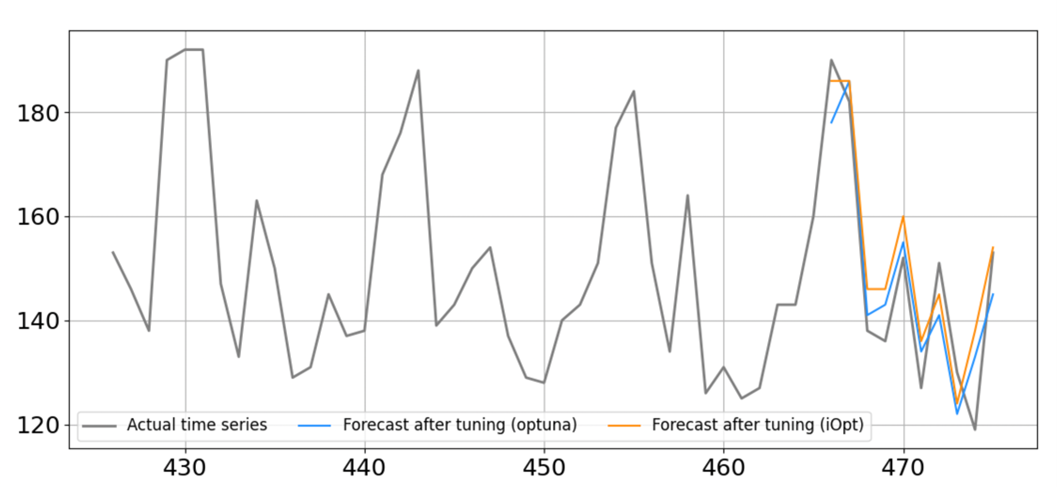
\includegraphics[width=1\textwidth]{fig3.png}
\caption{Prediction visualization.} \label{fig3}
\end{figure}
%
%
%
%TO DO: указать единицу измерения времени (секунды?)
%
%
%
\begin{table}
\centering
\caption{Results of solving the problem using iOpt and Optuna.}\label{tab1}
\begin{tabular}{|l|c|c|c|c|}
\hline
\multirow{2}{*}{P} & \multicolumn{2}{c|}{iOpt} & \multicolumn{2}{c|}{Optuna} \\
\cline{2-5} 
 & Solving time & Final $F_1$-score & Solving time & Final $F_1$-score \\
\hline
1 & 6574.2 & 13.5 & 9554.1 & 13.4 \\
2 & 3579.2 & 13.9 & 5127.5 & 13.6 \\
4 & 1998.7 & 13.6 & 2598.6 & 13.2 \\
8 & 1331.7 & 13.2 & 1275.4 & 13.2 \\
16 & 846.6 & 13.3 & 1148.5 & 13.3 \\
20 & 699.9 & 13.9 & 1578.6 & 13.3 \\
\hline
\end{tabular}
\end{table}

%(рус.) Ключевой характеристикой параллельных алгоритмов является ускорение. Мы будем использовать традиционное понятие ускорения как отношение времени последовательного запуска ко времени решения задачи в параллельном режиме. На Fig.3 приведены графики ускорения, полученного при параллельном запуске iOpt и OPTUNA. Наглядно видно, что iOpt на большом числе процессов показывает лучшее ускорение по сравнению с OPTUNA.
The key characteristic of parallel algorithms is speedup. We will use the traditional notion of speedup as the ratio of the time of sequential running to the time of solving the problem in the parallel mode. Fig.~\ref{fig4} and Fig.~\ref{fig5} show the graphs of speedup and time obtained by parallel running of iOpt and Optuna. We can clearly see that iOpt shows better speedup on a large number of processes compared to Optuna.

\begin{figure}
\center
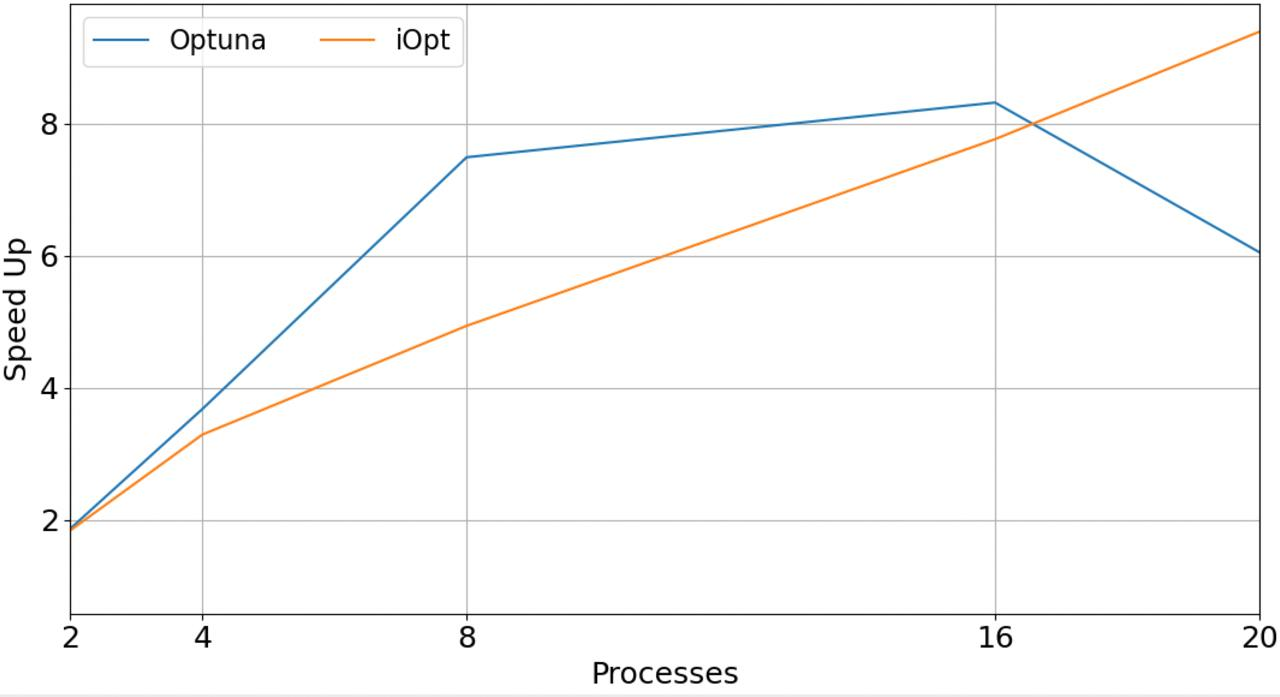
\includegraphics[width=0.8\textwidth]{fig4.png}
\caption{Speedup as a function of the number of processes.} \label{fig4}
\end{figure}

\begin{figure}
\center
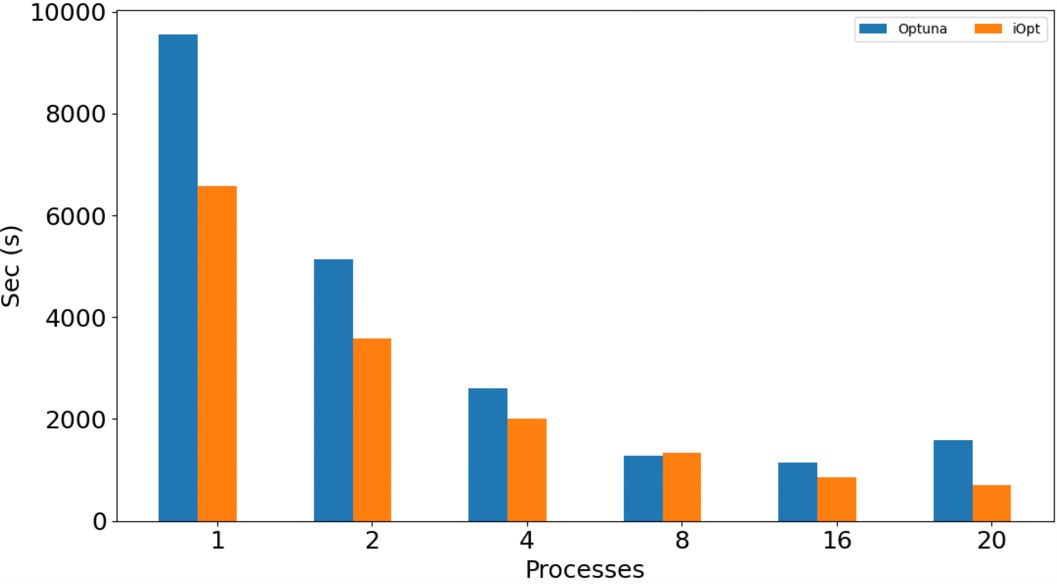
\includegraphics[width=0.8\textwidth]{fig5.png}
\caption{Solving time depending on the number of processes.} \label{fig5}
\end{figure}

\section{Conclusion}

%(рус.) Результаты экспериментов подтверждают, что алгоритм глобального поиска позволяет эффективно решать задачи настройки гиперпараметров методов искусственного интеллекта. Успешно обрабатываются ситуации, когда целевой критерий определен не всюду в области поиска. Параллельная программная реализация, выполненная в рамках iOpt solver, показывает хорошие ускорение и требует меньшего времени на решение задачи по сравнению с известными фреймворками для настройки гиперпараметров. 
Our experimental results confirm that the global search algorithm can effectively solve the problems of hyperparameter tuning for AI methods.  Situations when the objective criterion is not defined everywhere in the search domain are also handled successfully. The parallel software implementation within the iOpt solver shows a good speedup and requires less time to solve the problem compared to known frameworks for hyperparameter tuning.

%(рус.) Уменьшение прироста ускорения с ростом числа используемых процессов связана с необходимостью копирования большого объема данных, данная проблема будет решаться в дальнейшей работе. 
%(рус.) Для распараллеливания вычислений использовалась библиотека multiprocess, которая хорошо себя показывает при передаче небольших объемов данных между процессами, однако при увеличении количества процессов объем данных, которые необходимо скопировать растет линейно, из-за чего наблюдаем замедление роста ускорения с увеличением числа используемых процессов. Дальнейшие исследования будут направлены на повышение ускорения и поиск более эффективного алгоритма копирования и переиспользования данных.
To parallelize calculations in iOpt, we used the multiprocess library, which performs well when transferring small amounts of data between processes. However, when the number of parallel processes increases, the amount of data to be transferred between processes will grow linearly, which may cause the speedup to drop with the increasing number of processes being used. Further research will be geared towards  using a more efficient algorithm for copying and transferring data in iOpt in order to improve the speedup.


\begin{credits}
\subsubsection{\ackname} This study was supported by the Ministry of Science and Higher Education of the Russian Federation, project no. FSWR-2023-0034.

\subsubsection{\discintname}
The authors have no competing interests to declare that are relevant to the content of this article.
\end{credits}
%
% ---- Bibliography ----
%
% BibTeX users should specify bibliography style 'splncs04'.
% References will then be sorted and formatted in the correct style.
%
\bibliographystyle{splncs04}
\bibliography{bibliography}
%
%\begin{thebibliography}{8}
%\bibitem{ref_article1}
%Author, F.: Article title. Journal \textbf{2}(5), 99--110 (2016)
%
%\bibitem{ref_lncs1}
%Author, F., Author, S.: Title of a proceedings paper. In: Editor,
%F., Editor, S. (eds.) CONFERENCE 2016, LNCS, vol. 9999, pp. 1--13.
%Springer, Heidelberg (2016). \doi{10.10007/1234567890}
%
%\bibitem{ref_book1}
%Author, F., Author, S., Author, T.: Book title. 2nd edn. Publisher,
%Location (1999)
%
%\bibitem{ref_proc1}
%Author, A.-B.: Contribution title. In: 9th International Proceedings
%on Proceedings, pp. 1--2. Publisher, Location (2010)
%
%\bibitem{ref_url1}
%LNCS Homepage, \url{http://www.springer.com/lncs}, last accessed 2023/10/25
%\end{thebibliography}
\end{document}
